%%%%%%%%%%%%%%%%%%%%%%%%%%%%%%%%%%%%%%%%%%%%%%%%%%%%%%%%%%%%%%%%%%%%%%%%%%%%%%%%
%%%%%%%%%%%%%%%%%%%%%%%%%%%%%%%%%%%%%%%%%%%%%%%%%%%%%%%%%%%%%%%%%%%%%%%%%%%%%%%%
\chapter{Continuous Changes in the Power Grid}
\label{ch:appendix:sec:facts:simulations}
%%%%%%%%%%%%%%%%%%%%%%%%%%%%%%%%%%%%%%%%%%%%%%%%%%%%%%%%%%%%%%%%%%%%%%%%%%%%%%%%
%
This section is an extension of the~\cref{ch:facts} in which we consider
continuous changes to the power grid topology with the focus on the placement
of~\acrlong{facts} (\gls{facts}).
In~\cref{ch:appendix:sec:facts:fig:plot-cost-losses}, we investigate the
trade-off between costs and losses of the multi-objective function
(\cref{ch:facts:eq:objective}) that we optimize in our hybrid model
(\cref{ch:facts:lp:FCV-and-FCE}). In all our simulations, we see a Pareto front
that shows for different~$ \lambda \in [ 0,1 ] $ an optimal solution
in~\cref{ch:appendix:sec:facts:fig:plot-cost-losses}. 

If we concentrate on the placement problem, we can evaluate for different
numbers of control vertices~\glssymbol{factsbus} the operation costs for
different load increase factors. This is shown for different power grids
in~\cref{ch:appendix:sec:facts:plot-capacity-cost-controller}.
%
%
%%%%%%%%%%%%%%%%%%%%%%%%%%%%%%%%%%%%%%%%%%%%%%%%%%%%%%%%%%%%%%%%%%%%%%%%%%%%%%%%
\begingroup
\begin{figure}[t!]%
  \begin{subfigure}[t]{.45\textwidth}
    \centering
        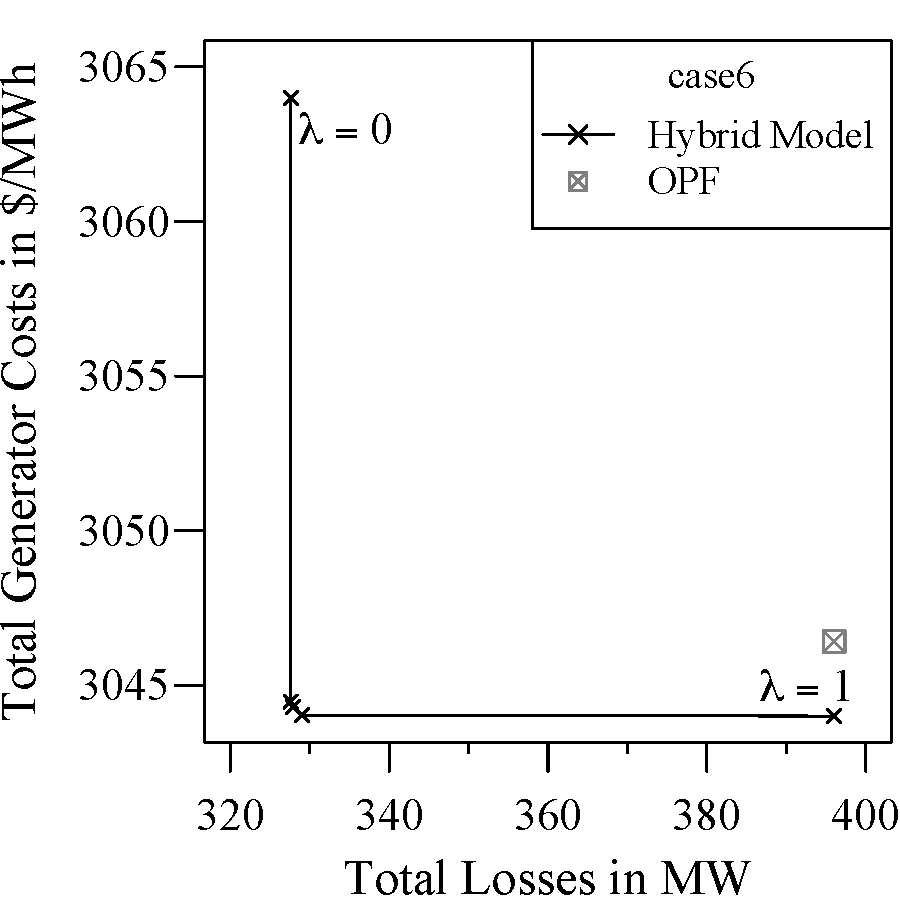
\includegraphics[width=0.95\linewidth, page=1,trim=0cm 0cm 0cm
        0cm]{factsplacement/plots/plotCostsVsLosses.pdf}
    \label{ch:appendix:sec:facts:fig:plot-costs-losses-case6}  
  \end{subfigure}
\hfill
  \begin{subfigure}[t]{.45\textwidth}
    \centering
        \includegraphics[width=0.95\linewidth, page=2,trim=0cm 0cm 0cm
        0cm]{factsplacement/plots/plotCostsVsLosses.pdf}
    \label{ch:appendix:sec:facts:fig:plot-costs-losses-case9}
\end{subfigure}

% \vspace{0.3cm}
\begin{subfigure}[t]{.45\textwidth}
    \centering
        \includegraphics[width=0.95\linewidth, page=3,trim=0cm 0cm 0cm
        0cm]{factsplacement/plots/plotCostsVsLosses.pdf}
\end{subfigure}
\hfill
\begin{subfigure}[t]{.45\textwidth}
    \centering
        \includegraphics[width=0.95\linewidth, page=5,trim=0cm 0cm 0cm 0cm]{factsplacement/plots/plotCostsVsLosses.pdf}
    \label{ch:appendix:sec:facts:fig:plot-costs-losses-case39}
\end{subfigure}

% \vspace{0.3cm}
\begin{subfigure}[t]{.45\textwidth}
    \centering
        \includegraphics[width=0.95\linewidth, page=6,trim=0cm 0cm 0cm 0cm]{factsplacement/plots/plotCostsVsLosses.pdf}
    \label{ch:appendix:sec:facts:fig:plot-costs-losses-case57}
\end{subfigure}
\hfill
\begin{subfigure}[b]{.45\textwidth}
    \centering
        \includegraphics[width=0.95\linewidth, page=7,trim=0cm 0cm 0cm 0cm]{factsplacement/plots/plotCostsVsLosses.pdf}
    \label{ch:appendix:sec:facts:fig:plot-costs-losses-case118}
\end{subfigure}
\vspace{0cm}
\caption{Trade-off of generator costs and costs of the losses
          depending as~$\lambda$ varies from~$0$ to~$1$. The square cross marks
          the solution computed by~\gls{opf}.}
\label{ch:appendix:sec:facts:fig:plot-cost-losses}
\end{figure}
%
%%%%%%%%%%%%%%%%%%%%%%%%%%%%%%%%%%%%%%%%%%%%%%%%%%%%%%%%%%%%%%%%%%%%%%%%%%%%%%%%
% \section{Grid Operation Under Increasing Loads}
\label{ch:facts:app:grid-control-when-approaching-capacity-limits}
%%%%%%%%%%%%%%%%%%%%%%%%%%%%%%%%%%%%%%%%%%%%%%%%%%%%%%%%%%%%%%%%%%%%%%%%%%%%%%%%
%
\newpage
\begin{figure}[t!]
\vspace{-1.4cm}
  \begin{subfigure}[t]{.45\textwidth}
    \centering
        \includegraphics[width=0.95\linewidth, page=3]{factsplacement/plots/plotCapacityReductionVsCostsController.pdf}
  \caption{case6.}
    \label{ch:appendix:sec:facts:fig:plot-capacity-cost-controller-case6}
\end{subfigure}
\hfill
\begin{subfigure}[t]{.45\textwidth}
    \centering
        \includegraphics[width=0.95\linewidth,
        page=4]{factsplacement/plots/plotCapacityReductionVsCostsController.pdf}
  \caption{case9.}
    \label{ch:appendix:sec:facts:fig:plot-capacity-cost-controller-case9}
\end{subfigure}

% \vspace{0.5cm}
\begin{subfigure}[t]{.45\textwidth}
    \centering
        \includegraphics[width=0.95\linewidth, page=5]{factsplacement/plots/plotCapacityReductionVsCostsController.pdf}
  \caption{case14.}
    \label{ch:appendix:sec:facts:fig:plot-capacity-cost-controller-case14}
\end{subfigure}
\hfill
\begin{subfigure}[t]{.45\textwidth}
    \centering
        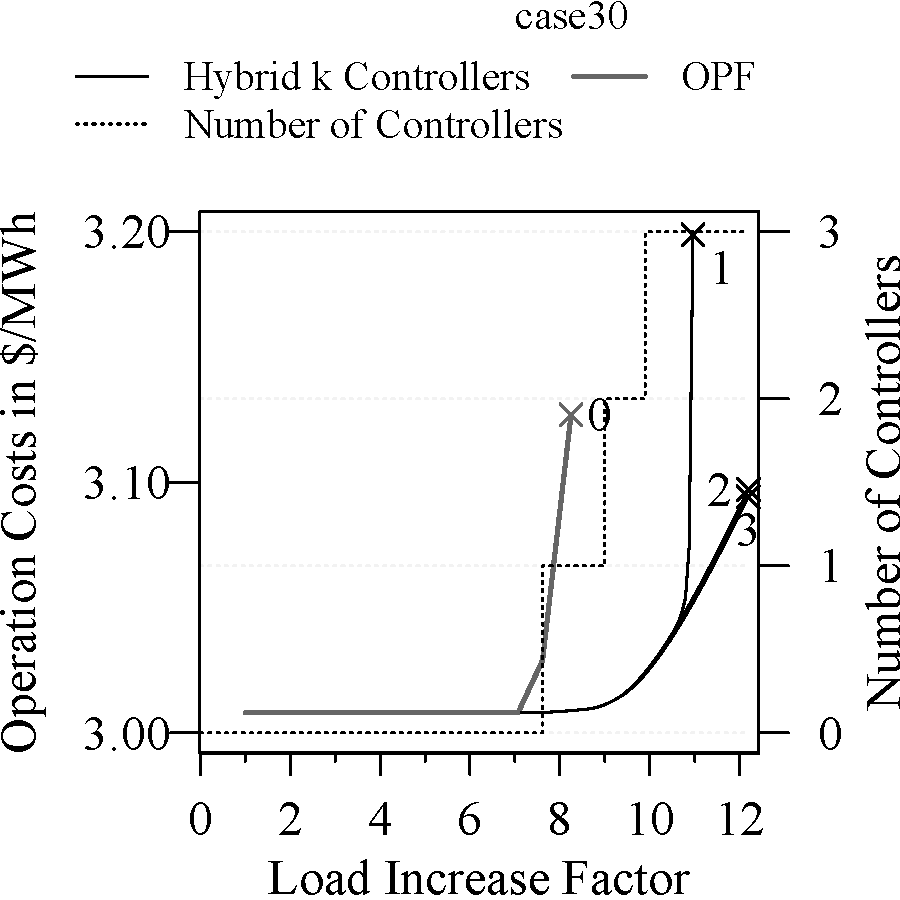
\includegraphics[width=0.95\linewidth, page=1]{factsplacement/plots/plotCapacityReductionVsCostsController.pdf}
  \caption{case30.}
    \label{ch:appendix:sec:facts:fig:plot-capacity-cost-controller-case30}
\end{subfigure}

% \vspace{0.5cm}
\begin{subfigure}[t]{.45\textwidth}
    \centering
        \includegraphics[width=0.95\linewidth, page=2]{factsplacement/plots/plotCapacityReductionVsCostsController.pdf}
  \caption{case39.}
    \label{ch:appendix:sec:facts:fig:plot-capacity-cost-controller-case39}
\end{subfigure}
\hfill
\begin{subfigure}[t]{.45\textwidth}
    \centering
        \includegraphics[width=0.95\linewidth, page=6]{factsplacement/plots/plotCapacityReductionVsCostsController.pdf}
    \caption{case118.}
    \label{ch:appendix:sec:facts:fig:plot-capacity-cost-controller-case118}
\end{subfigure}
\vspace{0cm}
    \caption{Operation costs of \texttt{case6} to \texttt{case118}
    for~\acrshort{opf} and the hybrid model with their control buses with
    respect to the load factor~$\rho$.}
\label{ch:appendix:sec:facts:plot-capacity-cost-controller}
\end{figure}
% 
\endgroup
% 